\chapter{Controle Bancário: Versão 3}\label{autorizacao}

Neste  capítulo,   dando  continuidade   ao  desenvolvimento  em   Grails,  será
apresentado o processo  de desenvolvimento da terceira versão  da aplicação {\bf
  ControleBancario}. Nessa versão são incorporadas as seguintes funcionalidades:

\begin{itemize}

\vspace{0.5cm}

\item Sintonia fina no controle de acesso:

\vspace{0.5cm}

\begin{itemize}

\vspace{0.5cm}

\item Atribuição de  papéis na criação das instâncias da  classe de domínio {\bf
  Gerente} e das instâncias das subclasses da classe {\bf Cliente}; 

\vspace{0.5cm}

\item Na segunda versão da  aplicação {\bf ControleBancario}, um cliente (físico
  ou jurídico)  pode acessar todas as  transações feitas em  contas (corrente ou
  poupança).  Na versão, discutida  nesse capítulo, clientes apenas terão acesso
  às transações realizadas nas contas (corrente ou poupança) a eles associadas;

\vspace{0.5cm}

\item  Se um  cliente possui  mais  de uma  conta (corrente  ou poupança),  será
  solicitado  que ele  escolha a  conta (corrente  ou poupança)  que  ele deseja
  acessar; 

\vspace{0.5cm}

\item Analogamente,  na segunda versão  da aplicação {\bf  ControleBancario}, um
  gerente  pode  acessar qualquer  conta  (corrente  ou  poupança).  Na  versão,
  discutida nesse capítulo, gerentes  apenas terão acesso às contas pertencentes
  à agência em que ele trabalha.

\end{itemize}

\vspace{0.5cm}

\item     Alteração     do    controlador     {\bf     Main},    definido     no
  Capítulo~\ref{autorizacao}, para refletir as mudanças relacionadas ao controle 
  de acesso;

\vspace{0.5cm}

\item  Alteração da  biblioteca  de marcas  {\it  LoginTagLibrary}, definida  no
  Capítulo~\ref{autorizacao}, para refletir as mudanças relacionadas ao controle
  de acesso; 

\vspace{0.5cm}

\item Acesso a um serviço {\it web}  que, dado um CEP como parâmetro, retorna as
  demais  informações de um  endereço (logradouro,  bairro, cidade,  etc). Essas
  informações  serão utilizadas  no  preenchimento automático  dos atributos  da
  classe de domínio {\bf Endereco}. 

\end{itemize}

\section{Configuração da aplicação} 

\vspace{0.5cm}

\noindent{\bf   Instalação   de    {\it   plugins}.}    Na   implementação   das
funcionalidades da aplicação  {\bf ControleBancario}, discutidas nesse capítulo,
será utilizado o {\it plugin}  Grails {\bf rest} que adiciona funcionalidades de
clientes REST. Ou  seja, ao utilizarmos esse {\it  plugin} será possível acessar
serviços web REST.\index{Plugins!rest} 

\begin{lstlisting}[numbers=left,  caption={\bf  BuildConfig.groovy}, frame=trBL,
    float=htbp, label=codBuildConfig3] 
grails.project.dependency.resolution = {
    // inherit Grails' default dependencies
    inherits("global") {
        // specify dependency exclusions here; for example, uncomment this to disable ehcache:
        // excludes 'ehcache'
    }
    log "error" // log level of Ivy resolver, either 'error', 'warn', 'info', 'debug' or 'verbose'
    checksums true // Whether to verify checksums on resolve
    legacyResolve false // whether to do a secondary resolve on plugin installation, not advised and 
                        // here for backwards compatibility

    repositories {
        inherits true // Whether to inherit repository definitions from plugins

        grailsPlugins()
        grailsHome()
        mavenLocal()
        grailsCentral()
        mavenCentral()
        // uncomment these (or add new ones) to enable remote dependency resolution from public Maven repositories
        mavenRepo "http://repository.codehaus.org"
        //mavenRepo "http://download.java.net/maven/2/"
        //mavenRepo "http://repository.jboss.com/maven2/"
        mavenRepo "http://repo.spring.io/milestone/"
    }

    dependencies {
        // specify dependencies here under either 'build', 'compile', 'runtime', 'test' or 'provided' scopes e.g.
        // runtime 'mysql:mysql-connector-java:5.1.27'
        runtime 'org.postgresql:postgresql:9.3-1100-jdbc41'
    }

    plugins {
        // plugins for the build system only
        build ":tomcat:7.0.50"

        // plugins for the compile step
        compile ":scaffolding:2.0.1"
        compile ':cache:1.1.1'

        // plugins needed at runtime but not for compilation
        runtime ":hibernate:3.6.10.7" // or ":hibernate4:4.1.11.6"
        runtime ":database-migration:1.3.8"
        runtime ":jquery:1.10.2.2"
        runtime ":resources:1.2.1"
        // Uncomment these (or add new ones) to enable additional resources capabilities
        //runtime ":zipped-resources:1.0.1"
        //runtime ":cached-resources:1.1"
        //runtime ":yui-minify-resources:0.1.5"
        
        compile ":br-validation:0.3"
        compile ":spring-security-core:2.0-RC2"
        compile ":rest:0.8"
    }
}
\end{lstlisting}

\vspace{1cm}

Para  instalar o  {\it  plugin} {\bf  rest}  adicione uma  linha, descrevendo  a
dependência, no  arquivo {\bf BuildConfig.groovy} conforme  apresentado na linha
53 do Código~\ref{codBuildConfig3}.  Porém, desde  que o código fonte desse {\it
  plugin}  encontra-se no  repositório da  {\it Codehaus},  é  necessário também
configurar  o endereço  desse repositório  conforme apresentado  na linha  21 do
Código~\ref{codBuildConfig3}.  

\newpage

\section{Atribuição de papéis}

\vspace{0.5cm}

Na   segunda  versão   da   aplicação  {\bf   ControleBancario},  discutida   no
Capítulo~\ref{autenticacao}, os papéis são  atribuídos durante o {\it Bootstrap}
da aplicação  (Código~\ref{codBootStrap23}). Nessa terceira  versão da aplicação
{\bf ControleBancario}, a atribuição de papéis seguirá a abordagem discutida nas
próximas seções. 

\subsection{Classe de domínio Gerente X Papel {\bf ROLE\_GERENTE}}

\vspace{0.5cm}

Na  terceira   versão  da  aplicação   {\bf  ControleBancario},  o   papel  {\bf
  ROLE\_GERENTE} será atribuído automaticamente às todas instâncias da classe de
domínio {\bf Gerente}.  

Código~\ref{codSaveGerente}  mostra a  reimplementação da  ação {\bf  save()} do
controlador {\bf GerenteController} com o objetivo de atribuir automaticamente o 
papel  {\bf ROLE\_GERENTE}  a  todas as  instâncias  da classe  de domínio  {\bf
  Gerente}. Conforme  pode-se observar,  logo após a  operação de {\bf  save} na
instância  da classe  de  domínio  {\bf Gerente}  (linha~27),  essa instância  é
associada ao papel {\bf ROLE\_GERENTE} (linhas~29-31). 

\begin{lstlisting}[numbers=left,  caption=Controlador {\bf  Gerente}  (ação {\bf
      save()}), frame=trBL, float=htbp, label=codSaveGerente] 
package br.ufscar.dc.dsw

import static org.springframework.http.HttpStatus.*
import grails.transaction.Transactional
import org.springframework.security.access.annotation.Secured

@Secured('ROLE_ADMIN')
@Transactional(readOnly = true)
class GerenteController {

    static allowedMethods = [save: "POST", update: "PUT", delete: "DELETE"]

    // Demais a^çõ^es/m^é^todos do controlador GerenteController

    @Transactional
    def save(Gerente gerenteInstance) {
        if (gerenteInstance == null) {
            notFound()
            return
        }

        if (gerenteInstance.hasErrors()) {
            respond gerenteInstance.errors, view:'create'
            return
        }

        gerenteInstance.save flush:true

        def gerentePapel = Papel.findByAuthority("ROLE_GERENTE")
        
        UsuarioPapel.create(gerenteInstance, gerentePapel)
        
        request.withFormat {
            form {
                flash.message = message(code: 'default.created.message', 
                                        args: [message(code: 'gerenteInstance.label', 
                                        default: 'Gerente'), gerenteInstance.id])
                redirect gerenteInstance
            }
            '*' { respond gerenteInstance, [status: CREATED] }
        }
    }
}
\end{lstlisting}

\newpage

\subsection{Classe de domínio Cliente X Papel {\bf ROLE\_CLIENTE}}

\vspace{0.5cm}

Analógo  ao  discutido na  seção  anterior,  o  papel {\bf  ROLE\_CLIENTE}  será
atribuído  automaticamente  às todas  instâncias  das  subclasses  da classe  de
domínio abstrata {\bf Cliente}.

\begin{lstlisting}[caption=Controlador {\bf  ClienteFisico} (ação {\bf save()}),
    frame=trBL, float=htbp, label=codSaveFisico] 
class ClienteFisicoController {

    // Demais a^çõ^es/atributos/m^é^todos do controlador ClienteFisicoController

    @Transactional
    def save(ClienteFisico clienteFisicoInstance) {
        if (clienteFisicoInstance == null) {
            notFound()
            return
        }
        if (clienteFisicoInstance.hasErrors()) {
            respond clienteFisicoInstance.errors, view:'create'
            return
        }

        clienteFisicoInstance.enabled = false       
        clienteFisicoInstance.save flush:true
        def clientePapel = Papel.findByAuthority("ROLE_CLIENTE")
        UsuarioPapel.create(clienteFisicoInstance, clientePapel)
        
        request.withFormat {
            form {
                flash.message = message(code: 'default.created.message', args: [message(code: 'clienteFisicoInstance.label', default: 'ClienteFisico'), clienteFisicoInstance.id])
                redirect clienteFisicoInstance
            }
            '*' { respond clienteFisicoInstance, [status: CREATED] }
        }
    }
}
\end{lstlisting}

Códigos~\ref{codSaveFisico}~e~\ref{codSaveJuridico} apresentam a reimplementação
da  ação {\bf  save()} dos  controladores {\bf  ClienteFisicoController}  e {\bf
  ClienteJuridicoController} com o objetivo  de atribuir automaticamente o papel
{\bf  ROLE\_CLIENTE}   a  todas  as   instâncias  da  classe  de   domínio  {\bf
  ClienteFisico} e {\bf ClienteJuridico}.  

\begin{lstlisting}[caption=Controlador   {\bf    ClienteJuridico}   (ação   {\bf
      save()}), frame=trBL, float=htbp, label=codSaveJuridico] 
class ClienteJuridicoController {

    // Demais a^çõ^es/atributos/m^é^todos do controlador ClienteJuridicoController

    @Transactional
    def save(ClienteJuridico clienteJuridicoInstance) {
        if (clienteJuridicoInstance == null) {
            notFound()
            return
        }
        if (clienteJuridicoInstance.hasErrors()) {
            respond clienteJuridicoInstance.errors, view:'create'
            return
        }

        clienteJuridicoInstance.enabled = false
        clienteJuridicoInstance.save flush:true
        def clientePapel = Papel.findByAuthority("ROLE_CLIENTE")
        UsuarioPapel.create(clienteJuridicoInstance, clientePapel)
       
        request.withFormat {
            form {
                flash.message = message(code: 'default.created.message', args: [message(code: 'clienteJuridicoInstance.label', default: 'ClienteJuridico'), clienteJuridicoInstance.id])
                redirect clienteJuridicoInstance
            }
            '*' { respond clienteJuridicoInstance, [status: CREATED] }
        }
    }
}
\end{lstlisting}

\newpage

\section{Controle de acesso: Transações}

\vspace{0.5cm}

Conforme  discutido no  Capítulo~\ref{autenticacao},  o acesso  às transações  é
restrito aos  usuários que desempenham  o papel {\bf ROLE\_CLIENTE}.  Porém essa
abordagem  não é suficiente  pois um  cliente pode  acessar todas  as transações
realizadas em contas (corrente ou poupança) independentemente se essa conta está
associada ou não a esse cliente.

Na  versão  da  aplicação  {\bf  ControleBancario},  discutida  nesse  capítulo,
clientes  apenas  terão  acesso  às  transações  realizadas  nas  contas  a  ele
associadas.  

\subsection{Controlador: MainController}

\vspace{0.5cm}

Conforme discutido, o controlador {\bf  MainController}, em conjunto com a visão
{\bf  index}   associada,  consiste  na  página  principal   da  aplicação  {\bf
  ControleBancario}. 

Código~\ref{codMainController2}  apresenta   a  reimplementação  da   ação  {\bf
  index()} do  controlador {\bf  MainController} com o  objetivo de  refletir as
mudanças relacionadas  a nova  abordagem de controle  de acesso  discutida nesse
capítulo. 

\begin{lstlisting}[caption=Controlador    {\bf    MainController},   frame=trBL,
    float=htbp, label=codMainController2, numbers=left] 
package br.ufscar.dc.dsw

import org.springframework.security.access.annotation.Secured

@Secured(['ROLE_ADMIN', 'ROLE_CLIENTE', 'ROLE_GERENTE'])
class MainController {

    def springSecurityService
    
    def index() { 
    
        def usuario = springSecurityService.getCurrentUser() 
        def authority = usuario.getAuthorities()[0].getAuthority()
        
        if (authority.equals('ROLE_GERENTE')) {
            if (!session.agencia) {
                session.agencia = usuario.agencia
                session.papel = "Gerente"
            }
        } else if (authority.equals('ROLE_CLIENTE')) {
            
            if (!session.papel) {
                session.papel = "Cliente"
            }
            
            if (!session.cliente) {
                session.cliente = usuario
            }
                        
            if (!session.contaCliente) {
                if (session.cliente.contasCliente.size() == 1) {
                    session.contaCliente = session.cliente.contasCliente[0]
                } else {
                    redirect(controller:'selecionaConta')
                }
            }
        } else {
            if (!session.papel) {
                session.papel = "Administrador"
            }
        }
    }
}
\end{lstlisting}

Quando um usuário acessa uma aplicação  {\it web}, ele estabelece uma sessão com
o servidor.  Uma variável de sessão existe  desde o instante de  sua criação até
que ela expire por inatividade, seja voluntariamente ({\it logout} da aplicação)
ou finalizado pela  aplicação.  Dessa forma, uma variável de  sessão é visível a
todos os controladores e visões enquanto não expirar por inatividade. 

\newpage

Conforme pode-se observar, quatro variáveis de sessão são utilizadas: 

\vspace{0.5cm}

\begin{itemize}

\item A variável de sessão {\bf papel}  armazena o nome do papel do usuário {\it
  logado} (linhas 18, 23 e 39); 

\vspace{0.5cm}

\item A  variável de sessão {\bf agencia}  armazena a agência em  que trabalha o
  usuário {\it logado}, caso este  desempenhe o papel {\bf ROLE\_GERENTE} (linha
  17); 

\vspace{0.5cm}

\item A variável  de sessão {\bf cliente} armazena o  usuário {\it logado}, caso
  este desempenhe o papel {\bf ROLE\_CLIENTE} (linha 27); e 

\vspace{0.5cm}

\item  A  variável  de  sessão  {\bf  contaCliente}  armazena  a  conta  cliente
  (instância  da  classe de  domínio  {\bf  ContaCliente})  que o  usuário  {\it
  logado}, caso este  desempenhe o papel {\bf ROLE\_CLIENTE},  está acessando no
  momento.  Se  o cliente  possuir  apenas uma  conta  associada,  este já  será
  armazenado  na  variável  de  sessão  {\bf  contaCliente}  (linha  32).   Caso
  contrário,    há    um    redirecionamento    para    o    controlador    {\bf
    SelecionaContaController} (linha 34).  

\end{itemize}

\subsection{Biblioteca de marcas: LoginTagLib}

\vspace{0.5cm}

No Código~\ref{codTagLib2}  tem-se a biblioteca de marcas  {\bf LoginTagLib} que
foi reimplementada para refletir as alterações discutidas nesse capítulo.  

Conforme pode-se observar essa classe  imprime o nome do papel desempenhado pelo
usuário {\it  logado} (variável de sessão  {\bf papel}, linha  23).  Além disso,
essa  classe  imprime  a  conta  que  o usuário  {\it  logado}  está  acessando,
considerando que esse desempenhe o papel {\bf ROLE\_CLIENTE} (variável de sessão
{\bf contaCliente}, linha 15).  

Por fim, essa  classe imprime a agência em que o  usuário {\it logado} trabalha,
caso  esse desempenhe  o  papel  {\bf ROLE\_GERENTE}  (variável  de sessão  {\bf
  agencia}, linha 19).  

\begin{lstlisting}[caption=Biblioteca  de marca  {\bf  LoginTagLib}, frame=trBL,
    float=htbp, label=codTagLib2, numbers=left] 
class LoginTagLib {
    def springSecurityService
    def loginControl = {
        if (springSecurityService.isLoggedIn()) {
            def usuario = springSecurityService.getCurrentUser() 
            def authority = usuario.getAuthorities()[0].getAuthority()
            def papel
            
            def span = "<span style=\"text-align:center;padding-left:25px;padding-right:25px\">"
            
            StringBuilder sb = new StringBuilder();
            
            if (session.contaCliente) {
                sb.append("Conta: ")
                sb.append(session.contaCliente.conta + " [")
                sb.append(session.contaCliente.conta.agencia + "]")
                sb.append(span)
            } else if (session.agencia) { 
                sb.append("Ag^ê^ncia: ")
                sb.append(session.agencia)
            }
            
            out << span
            out << session.papel
            out << "</span>"
            out << span
            out << sb
            out << "</span>"
            out << "<span style=\"padding-right:25px\">"
            out << """ [${link(controller: "logout"){"Logout"}}]"""
            out << "</span>"
        }
    }
}
\end{lstlisting}

\subsection{Controlador: SelecionaContaController}\label{secSeleciona}

\vspace{0.5cm}

Caso um  cliente possua  mais de  uma conta (corrente  ou poupança),  ele deverá
escolher que  conta (corrente  ou poupança) ele  deseja acessar.   O controlador
{\bf SelecionaContaController}  é responsável  por essa nova  funcionalidade.  A
implementação      desse     controlador     encontra-se      apresentada     no
Código~\ref{codSelecionaContaController}.  

\vspace{0.2cm}

\begin{itemize}

\item  A ação  {\bf index()}  simplesmente  invoca implicitamente  a visão  {\bf
  index.gsp} que será discutida na próxima seção; e

\vspace{0.2cm}

\item A ação {\bf selected()} é  responsável por: (1) receber, como parâmetro, a
  conta escolhida pelo  usuário {\it logado} e armazenar  essa conta na variável
  de  sessão  {\bf  contaCliente}  e   (2)  redirecionar  a  requisição  para  o
  controlador {\bf MainController}. 

\end{itemize}

\begin{lstlisting}[caption=Controlador      {\bf      SelecionaContaController},
    frame=trBL, float=htbp, label=codSelecionaContaController] 
package br.ufscar.dc.dsw 
import org.springframework.security.access.annotation.Secured

@Secured('ROLE_CLIENTE')
class SelecionaContaController {

    def index() { }
    
    def selected() {        
        session.contaCliente = ContaCliente.get(params.conta)
        redirect(controller:'main')
    }
}
\end{lstlisting}

\subsection{Visão: selecionaConta/index.gsp}

\vspace{0.5cm}

Relembrando   a   discussão  da   Seção~\ref{secEstatico},   para  cada   método
correspondente a  uma ação em um  controlador é criada  uma correspondente visão
(arquivo  com  extensão {\bf  .gsp}).   Assim, a  ação  {\bf  index()}, de  {\bf
  SelecionaContaController}, tem o correspondente {\bf index.gsp}.  

A visão  {\bf index.gsp}  cria um formulário  HTML com  um campo de  seleção que
contém as contas clientes associadas ao cliente {\it logado} (variável de sessão
{\bf cliente}).  É  importante salientar que a submissão  do formulário invoca a
ação   {\bf   selected()}    do   controlador   {\bf   SelecionaContaController}
(Seção~\ref{secSeleciona}). A implementação  dessa visão encontra-se apresentada
no Código~\ref{codSelecionaContaIndex}.  

\begin{lstlisting}[caption=Visão   {\bf  selecionaConta/index.gsp},  frame=trBL,
    float=htbp, label=codSelecionaContaIndex] 
<%@ page import="br.ufscar.dc.dsw.ContaCliente" %>
<!DOCTYPE html>
<html>
    <head>
        <meta name="layout" content="main">
    </head>
    <body>
        <div id="status" role="complementary">
            <h1>Selecione Conta:</h1>
            <g:form url="[action:'selected']" >
                <g:set var="contas" value="${ContaCliente.findAll("from ContaCliente as contaCliente where contaCliente.cliente = ?", [session.cliente])}" />
                <g:select name="conta" from="${contas}" 
                    optionKey="id" optionValue="conta">
                </g:select>
                </br>
                </br>
                <fieldset class="buttons">
                    <g:submitButton name="OK" class="save" value="OK" />
                </fieldset>
            </g:form>
        </div>
    </body>
</html>
\end{lstlisting}

\subsection{Classe de Domínio: Transacao}

\vspace{0.5cm}

Código~\ref{codTransacao2} mostra  a reimplementação  da classe de  domínio {\bf
  Transacao} com o  objetivo de refletir as mudanças  discutidas nesse capítulo.
Por questão de brevidade, apenas serão apresentadas as mudanças realizadas nessa
classe  de domínio.   Conforme pode-se  observar, foram  definidos  dois métodos
({\bf  getValorReal()} e  {\bf getValorAnterior()})  que serão  utilizados pelas
ações  {\bf  save()},  {\bf  update()}  e {\bf  delete()}  do  controlador  {\bf
  TransacaoController}.  

\begin{lstlisting}[caption=Classe  de  domínio {\bf  Transacao},  frame =  trBL,
    float=htbp, label=codTransacao2] 
class Transacao {
    
    // Demais atributos/m^é^todos da classe de dom^í^nio Transacao

    static transients = ['valorAnterior', 'valorReal']
    
    double getValorReal() { // Retorna valor negativo caso transa^çã^o seja um d^é^bito
        return (tipo == D^É^BITO) ? -valor : valor;
    }
    
    double getValorAnterior() {
        def ant = this.getPersistentValue('valor') // Retorna o valor do atributo 'valor' antes de ser persistido
        def tipo = this.getPersistentValue('tipo') // Retorna o valor do atributo 'tipo' antes de ser persistido
        if (tipo == Transacao.D^É^BITO) {
            ant = -ant // Retorna valor negativo caso transa^çã^o seja um d^é^bito
        }
        return ant
    } 
}
\end{lstlisting}

\subsection{Controlador: TransacaoController}\label{secTransacaoController2}

\vspace{0.5cm}

Código~\ref{codTransacaoController3}  mostra  a  reimplementação do  controlador
{\bf TransacaoController} com o objetivo  de refletir as mudanças relacionadas a
nova abordagem de  controle de acesso discutida nesse  capítulo.  Por questão de
brevidade, apenas serão apresentadas as mudanças realizadas nesse controlador.  

Relembrando  a  discussão  da  Seção~\ref{secTransacaoController}, a  ação  {\bf
  index()} é responsável por retornar a lista de instâncias da classe de domínio
{\bf Transacao}.  No caso da implementação apresentada nesse capítulo, a lista é
composta  apenas  pelas  transações  que  foram realizadas  na  conta  escolhida
anteriormente pelo usuário {\it logado} (variável de sessão {\bf contaCliente}).  

A ação {\bf create()} é responsável por criar uma instância da classe de domínio
{\bf Transacao} que  é repassada (retornada) para a  visão {\bf create.gsp} (uma
página que contem  um formulário HTML). Quando o formulário  é submetido, a ação
{\bf save()} valida  os dados e caso, tenha sucesso, grava  a instância no banco
de dados e  redireciona para a ação  {\bf show()}.  Por outro lado,  se os dados
são inválidos, a ação {\bf  save()} renderiza a visão {\bf create.gsp} novamente
para  que o  usuário  corriga os  erros  encontrados na  validação.  No caso  da
implementação apresentada nesse capítulo, a transação criada é associada à conta
escolhida  anteriormente pelo  usuário  {\it logado}  (variável  de sessão  {\bf
  contaCliente}).  

Analogamente, a  ação {\bf edit()} é  responsável por recuperar  uma instância a
ser atualizada  posteriormente.  A instância recuperada  é repassada (retornada)
para a visão {\bf edit.gsp} (uma página que contém um formulário HTML). Quanto o
formulário é  submetido o método  {\bf update()} valida  os dados e  caso, tenha
sucesso, atualiza a  instância no banco de dados e redireciona  para a ação {\bf
  show()}.  Por  outro lado, se  os dados são  inválidos, a ação  {\bf update()}
renderiza a visão  {\bf edit.gsp} novamente para que o  usuário corriga os erros
encontrados na  validação.  É importante salientar  que as ações  {\bf save()} e
{\bf  update()}  atualizam  o  saldo   da  conta  para  refletir  as  transações
criadas e/ou atualizadas. 

\begin{lstlisting}[caption=Controlador  {\bf  TransacaoController},  frame=trBL,
    float=htbp, label=codTransacaoController3] 
class TransacaoController {

    // Demais a^çõ^es/atributos/m^é^todos do controlador TransacaoController

    def index(Integer max) {
        params.max = Math.min(max ?: 10, 100)
        def results = Transacao.findAllByContaCliente(session.contaCliente, params)
        respond results, model:[transacaoInstanceCount: Transacao.count()]
    }

    @Transactional
    def save(Transacao transacaoInstance) {
        if (transacaoInstance == null) {
            notFound()
            return
        }
        if (transacaoInstance.hasErrors()) {
            respond transacaoInstance.errors, view:'create'
            return
        }
        def conta = transacaoInstance.contaCliente.conta        
        conta.saldo += transacaoInstance.getValorReal()
        transacaoInstance.save flush:true
        conta.save flush:true

        request.withFormat {
            form {
                flash.message = message(code: 'default.created.message', args: [message(code: 'transacaoInstance.label', default: 'Transacao'), transacaoInstance.id])
                redirect transacaoInstance
            }
            '*' { respond transacaoInstance, [status: CREATED] }
        }
    }


    def edit(Transacao transacaoInstance) {                
        if (transacaoInstance != null && transacaoInstance.contaCliente.id != session.contaCliente.id) {
            flash.message = message(code: 'springSecurity.denied.message', args: [message(code: 'Transacao.label', default: 'Transacao'), transacaoInstance.id])
            redirect action: "index"
        }
        respond transacaoInstance
    }

    @Transactional
    def update(Transacao transacaoInstance) {
        if (transacaoInstance == null) {
            notFound()
            return
        }
        if (transacaoInstance.hasErrors()) {
            respond transacaoInstance.errors, view:'edit'
            return
        }
        def conta = transacaoInstance.contaCliente.conta        
        conta.saldo += (transacaoInstance.getValorReal() - transacaoInstance.getValorAnterior())
        transacaoInstance.save flush:true
        conta.save flush:true
        
        request.withFormat {
            form {
                flash.message = message(code: 'default.updated.message', args: [message(code: 'Transacao.label', default: 'Transacao'), transacaoInstance.id])
                redirect transacaoInstance
            }
            '*'{ respond transacaoInstance, [status: OK] }
        }
    }

    @Transactional
    def delete(Transacao transacaoInstance) {                
        if (transacaoInstance.contaCliente.id != session.contaCliente.id) {
            flash.message = message(code: 'springSecurity.denied.message', args: [message(code: 'Transacao.label', default: 'Transacao'), transacaoInstance.id])
            redirect action: "index", method: "GET"
            return
        }
        if (transacaoInstance == null) {
            notFound()
            return
        }
        def conta = transacaoInstance.contaCliente.conta;
        conta.saldo -= transacaoInstance.getValorReal()
        transacaoInstance.delete flush:true
        conta.save flush:true

        request.withFormat {
            form {
                flash.message = message(code: 'default.deleted.message', args: [message(code: 'Transacao.label', default: 'Transacao'), transacaoInstance.id])
                redirect action:"index", method:"GET"
            }
            '*'{ render status: NO_CONTENT }
        }
    }
}
\end{lstlisting}

\newpage

Relembrando  a discussão da  Seção~\ref{secURL}, Grails  usa uma  convenção para
automaticamente configurar o caminho para uma ação em particular. Por exemplo, a
URL  \url{http://localhost:8080/ControleBancario/transacao/edit/1}  executaria a
ação {\bf  edit()} na instância da  classe de domínio {\bf  Transacao} cujo {\bf
  id} é igual a 1. 

Dessa forma, através da digitação de  uma URL no navegador {\it web}, um cliente
{\it logado} pode editar ou remover indevidamente (maliciosamente) uma transação
não associada a nenhuma de suas  contas. Nesse contexto, as ações {\bf edit()} e
{\bf delete()}  foram alteradas  com o objetivo  de prevenir  essas atualizações
indevidas.  Por  fim, a  ação {\bf  delete()} também atualiza  o saldo  da conta
associada (crédito ou débito) para refletir a operação de remoção da transação.

\subsection{Template transacao/\_form.gsp}

\vspace{0.5cm}

O {\it template}  {\bf \_form.gsp}, utilizado tanto pela  visão {\bf create.gsp}
quanto  pela  visão   {\bf  edit.gsp},  representa  os  campos   que  devem  ser
preenchidos/alterados  durante a  criação/edição  de instâncias  das classes  de
domínio. 

Código~\ref{codTransacaoForm}  mostra as mudanças  realizadas no  {\it template}
{\bf  transacao/\_form.gsp} para  refletir às  novas  funcionalidades discutidas
nesse capítulo. Por questão de  brevidade, apenas serão apresentadas as mudanças
realizadas nesse arquivo.  

\begin{lstlisting}[caption={\it     Template}     {\bf    transacao/\_form.gsp},
    frame=trBL, float=htbp, label=codTransacaoForm, numbers=left]
<%@ page import="br.ufscar.dc.dsw.CaixaEletronico" %>
<%@ page import="br.ufscar.dc.dsw.Transacao" %>

<div class="fieldcontain ${hasErrors(bean: transacaoInstance, field: 'contaCliente', 'error')} required">
	<label for="contaCliente">
		<g:message code="transacao.contaCliente.label" default="Conta Cliente" />
		<span class="required-indicator">*</span>
	</label>

	<g:select id="contaCliente" name="contaCliente.id" from="${session.contaCliente}" optionKey="id" 
            required="" value="${transacaoInstance?.contaCliente?.id}" class="many-to-one"/>
</div>

<div class="fieldcontain ${hasErrors(bean: transacaoInstance, field: 'caixaEletronico', 'error')} ">
	<label for="caixaEletronico">
		<g:message code="transacao.caixaEletronico.label" default="Caixa Eletronico" />
		<span class="required-indicator">*</span>
	</label>
        
  <g:set var="caixas" value="${CaixaEletronico.findAll("from CaixaEletronico as caixa where caixa.banco = ?", 
         [session.contaCliente.conta.agencia.banco])}" />
	<g:select id="caixaEletronico" name="caixaEletronico.id" from="${caixas}" optionKey="id" 
            value="${transacaoInstance?.caixaEletronico?.id}" class="many-to-one" />
</div>

<%-- Nenhuma altera^çã^o nos demais campos -->

\end{lstlisting}

Basicamente   foram  realizadas   duas   alterações  no   {\it  template}   {\bf
  transacao/\_form.gsp}. A  primeira consiste em  alterar o atributo  {\bf from}
(linha  10) do  campo de  seleção de  tal forma  que a  transação criada/editada
sempre  será associada à  conta escolhida  anteriormente pelo  usuário (variável
sessão {\bf contaCliente}).  

A segunda alteração consiste em modificar  o segundo campo de seleção (linha 22)
de  tal  forma  que  o  usuário  {\it logado}  apenas  possa  selecionar  caixas
eletrônicos pertencentes  ao banco que mantém  a conta (variável  de sessão {\bf
  contaCliente})  sendo  acessada  no  momento.  É importante  salientar  que  o
atributo  {\bf from}  desse  campo de  seleção  é a  variável  {\bf caixas}  que
armazena  uma lista  de instâncias  da classe  de domínio  {\bf CaixaEletronico}
obtida  através da  execução  de  uma consulta  {\bf  findAll()} (linhas  20-21)
parametrizada. O  parâmetro dessa consulta  é o banco  que mantém a  conta sendo
acessada no momento.

\subsection{Executando a aplicação}

\vspace{0.5cm}

Após realizar  as alterações discutidas  nessa seção, sugere-se que  a aplicação
{\bf ControleBancario} seja executada. 

Figura~\ref{figPageCliente} apresenta  a página principal  conforme acessada por
um usuário {\it logado} que desempenha o papel {\bf ROLE\_CLIENTE}. 

\begin{figure}[htbp]
\centering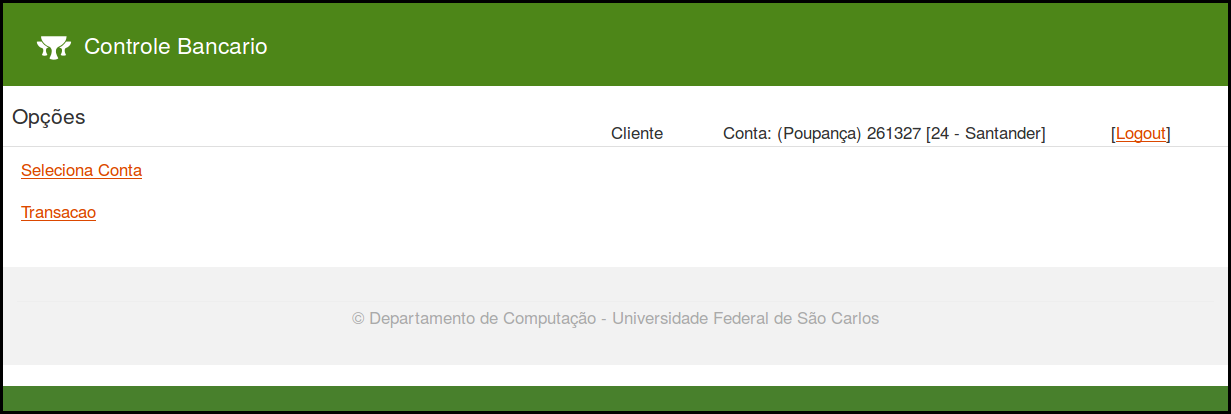
\includegraphics[width=13cm]{pageCliente}
\caption{Visão {\bf main/index.gsp}: {\bf ROLE\_CLIENTE}}
\label{figPageCliente}
\end{figure}

Conforme pode-se  observar o  usuário {\it logado}  tem duas  opções disponíveis
(dois controladores da aplicação {\bf ControleBancario}):

\vspace{0.3cm}

\begin{itemize}

\item {\bf SelecionaConta} caso deseje escolher que conta (corrente ou poupança)
  ele deseja acessar;

\vspace{0.3cm}

\item  {\bf  Transacao} caso  deseje  acessar/atualizar  a  lista de  transações
  realizadas    na    conta    que    está   sendo    acessada    no    momento.
  Figura~\ref{indexTransacaoFig}  apresenta a lista  de transações  associadas a
  uma conta do usuário {\it logado}.  

\end{itemize}

\begin{figure}[htbp]
\centering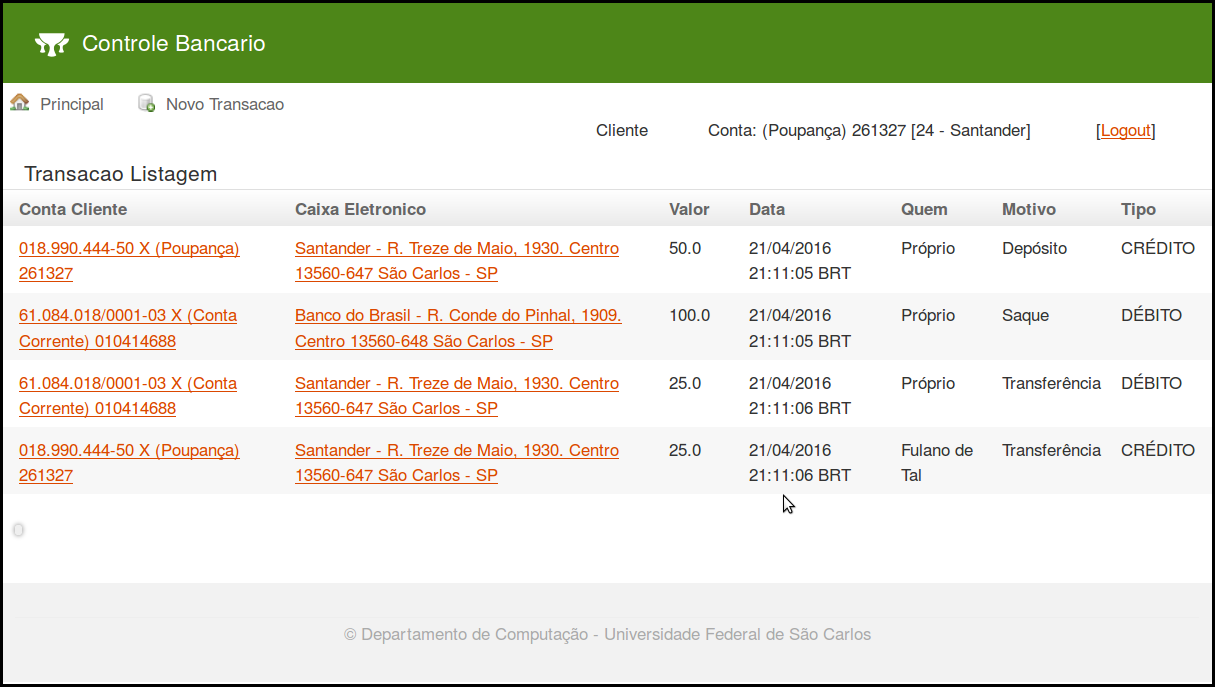
\includegraphics[width=13cm]{indexTransacao}
\caption{Lista de transações de uma conta do usuário {\it logado}}
\label{indexTransacaoFig}
\end{figure}

\section{Controle de acesso: Contas}

\vspace{0.5cm}

Conforme discutido no Capítulo~\ref{autenticacao}, o acesso às contas é restrito
aos usuários que desempenham o  papel {\bf ROLE\_GERENTE}.  Porém essa abordagem
não  é suficiente  pois um  gerente pode  acessar todas  as contas  (corrente ou
poupança) independentemente se essa conta pertence ou não a sua agência.

Na  versão  da  aplicação  {\bf  ControleBancario},  discutida  nesse  capítulo,
gerentes  apenas  terão acesso  às  contas pertencentes  à  agência  em que  ele
trabalha. 

\subsection{Controlador: ContaCorrenteController}

\vspace{0.5cm}

Código~\ref{codContaCorrenteController}    apresenta   a    reimplementação   do
controlador {\bf ContaCorrenteController} com o objetivo de refletir as mudanças
relacionadas a nova abordagem de controle de acesso discutida nesse capítulo.  

Relembrando  a  discussão  da  Seção~\ref{secTransacaoController}, a  ação  {\bf
  index()} é responsável por retornar a lista de instâncias da classe de domínio
{\bf  ContaCorrente}.  No caso  da implementação  apresentada nesse  capítulo, a
lista é composta apenas pelas contas  correntes que pertencem à agência em que o
usuário {\it logado} trabalha (variável de sessão {\bf agencia}). 

Por  fim,  relembrando  a  discussão da  Seção~\ref{secTransacaoController2},  é
possível que  gerentes {\it logados}  acessem de forma indevida  (maliciosa) uma
conta não  associada à agência  em que trabalha.  Nesse contexto, as  ações {\bf
  edit()}  e {\bf delete()}  foram alteradas  com o  objetivo de  prevenir essas
atualizações indevidas.

\vspace{0.5cm}

\begin{remark}
Análogo  ao  controlador   {\bf  ContaCorrenteController},  o  controlador  {\bf
  ContaPoupancaController}  também  necessita  ser  alterado  para  refletir  as
mudanças relacionadas  a nova  abordagem de controle  de acesso  discutida nesse
capítulo. Fica como exercício para o leitor realizar tal alteração.
\end{remark}

\subsection{Template contaCorrente/\_form.gsp}

\vspace{0.5cm}

O {\it template}  {\bf \_form.gsp}, utilizado tanto pela  visão {\bf create.gsp}
quanto  pela  visão   {\bf  edit.gsp},  representa  os  campos   que  devem  ser
preenchidos/alterados  durante a  criação/edição  de instâncias  das classes  de
domínio. 

Código~\ref{codContaCorrenteForm}  apresenta  as  mudanças  realizadas  no  {\it
  template}    {\bf   contaCorrente/\_form.gsp}    para   refletir    às   novas
funcionalidades  discutidas nesse  capítulo.  Por questão  de brevidade,  apenas
serão apresentadas as mudanças realizadas nesse arquivo.

Basicamente  foi   realizada  apenas  uma  alteração  no   {\it  template}  {\bf
  contaCorrente/\_form.gsp} e  consiste em alterar atributo {\bf  from} do campo
de  seleção  de  tal forma  que  a  conta  corrente criada/editada  sempre  será
associada à agência (variável de sessão {\bf agencia}) em que trabalha o usuário
{\it logado}.

\vspace{0.5cm}
 
\begin{remark}
Análogo ao {\it template}  {\bf contaCorrente/\_form.gsp}, o {\it template} {\bf
  contaPoupanca/\_form.gsp}  também  precisa  ser  alterado  com  o  intuito  de
desabilitar  o campo  de seleção  ({\bf Agência}).  Fica como  exercício  para o
leitor realizar tal alteração. 
\end{remark}

\begin{lstlisting}[caption=Controlador       {\bf      ContaCorrenteController},
    frame=trBL, float=htbp, label=codContaCorrenteController] 
class ContaCorrenteController {

    // Demais a^çõ^es/atributos/m^é^todos do controlador ContaCorrenteController

    def index(Integer max) {
        params.max = Math.min(max ?: 10, 100)        

        def results = ContaCorrente.findAllByAgencia(session.agencia, params)

        respond results, model:[contaCorrenteInstanceCount: ContaCorrente.count()]
    }

    def edit(ContaCorrente contaCorrenteInstance) {
        
        if (contaCorrenteInstance != null && contaCorrenteInstance.agencia.id != session.agencia.id) {
            flash.message = message(code: 'springSecurity.denied.message', args: [message(code: 'transacaoInstance.label', default: 'Transacao'), contaCorrenteInstance.id])
            redirect action: "index"
        }

        respond contaCorrenteInstance
    }

    @Transactional
    def delete(ContaCorrente contaCorrenteInstance) {
        
        if (contaCorrenteInstance.agencia.id != session.agencia.id) {
            flash.message = message(code: 'springSecurity.denied.message', args: [message(code: 'transacaoInstance.label', default: 'Transacao'), contaCorrenteInstance.id])
            redirect action: "index"
            return
        }

        if (contaCorrenteInstance == null) {
            notFound()
            return
        }

        contaCorrenteInstance.delete flush:true

        request.withFormat {
            form {
                flash.message = message(code: 'default.deleted.message', args: [message(code: 'ContaCorrente.label', default: 'ContaCorrente'), contaCorrenteInstance.id])
                redirect action:"index", method:"GET"
            }
            '*'{ render status: NO_CONTENT }
        }
    }
}
\end{lstlisting}

\begin{lstlisting}[caption={\it    Template}   {\bf   contaCorrente/\_form.gsp},
    frame=trBL, float=htbp, label=codContaCorrenteForm]
<%@ page import="br.ufscar.dc.dsw.ContaCorrente" %>

<div class="fieldcontain ${hasErrors(bean: contaCorrenteInstance, field: 'agencia', 'error')} required">
	<label for="agencia">
		<g:message code="contaCorrente.agencia.label" default="Agencia" />
		<span class="required-indicator">*</span>
	</label>
	<g:select id="agencia" name="agencia.id" from="${session.agencia}" optionKey="id" required="" value="${contaCorrenteInstance?.agencia?.id}" disabled class="many-to-one"/>
</div>

<%-- Nenhuma altera^çã^o nos demais campos -->

\end{lstlisting}

\subsection{Controlador: ContaClienteController}

\vspace{0.5cm}

Código~\ref{codContaClienteController2}    apresenta   a    reimplementação   do
controlador {\bf ContaClienteController} com o objetivo de refletir as mudanças
relacionadas a nova abordagem de controle de acesso discutida nesse capítulo.  

A ação {\bf index()} é responsável  por retornar a lista de instâncias da classe
de   domínio  {\bf   ContaCliente}   que  materializa   o  relacionamento   {\em
  muitos-para-muitos}  entre   as  classes  de   domínio  {\bf  Conta}   e  {\bf
  Cliente}.   No  caso da  implementação  apresentada  nessa  seção, a  lista  é
composta apenas pelas  instâncias que estão associadas a  contas que pertencem à
agência  em  que  o usuário  {\it  logado}  trabalha  (variável de  sessão  {\bf
  agencia}).  

A ação {\bf save()} valida os dados  e caso, tenha sucesso, grava a instância no
banco de  dados. No caso da  implementação apresentada nessa seção,  a ação {\bf
  save()}  também habilita  o cliente  (torna-se um  usuário da  aplicação) caso
esteja desabilitado. No contexto da aplicação {\bf ControleBancario}, um cliente
apenas  torna-se  um  usuário (pode  realizar  a  operação  de {\it  login})  da
aplicação caso tenha uma conta associada. 

Além  disso, conforme  discutido  anteriormente, é  possível  que gerentes  {\it
  logados}  acessem de  forma indevida  (maliciosa) instâncias  dessa  classe de
domínio.  Nesse contexto, as ações {\bf edit()} e {\bf delete()} foram alteradas
com o objetivo de prevenir essas atualizações indevidas. 

\begin{lstlisting}[caption=Controlador {\bf ContaClienteController}, frame=trBL,
    float=htbp, label=codContaClienteController2] 
class ContaClienteController {

    // Demais a^çõ^es/atributos/m^é^todos do controlador ContaClienteController

    def index(Integer max) {
        params.max = Math.min(max ?: 10, 100)
		
        def results = ContaCliente.findAll("from ContaCliente as cc where cc.conta.agencia = :agencia",
            [agencia: session.agencia])
		
        respond results, model:[contaClienteInstanceCount: ContaCliente.count()]
    }

    @Transactional
    def save(ContaCliente contaClienteInstance) {
        if (contaClienteInstance == null) {
            notFound()
            return
        }

        if (contaClienteInstance.hasErrors()) {
            respond contaClienteInstance.errors, view:'create'
            return
        }

        contaClienteInstance.save flush:true

        def clienteInstance = contaClienteInstance.cliente 

        if (!clienteInstance.enabled) {
            clienteInstance.enabled = true
            clienteInstance.save flush:true
        }
        
        request.withFormat {
            form {
                flash.message = message(code: 'default.created.message', args: [message(code: 'contaClienteInstance.label', default: 'ContaCliente'), contaClienteInstance.id])
                redirect contaClienteInstance
            }
            '*' { respond contaClienteInstance, [status: CREATED] }
        }
    }
}
\end{lstlisting}

\newpage

\subsection{Template contaCliente/\_form.gsp}

\vspace{0.5cm}

Código~\ref{codContaClienteForm}  apresenta  as   mudanças  realizadas  no  {\it
  template}  {\bf transacao/\_form.gsp} para  refletir às  novas funcionalidades
discutidas nesse  capítulo. Por questão de brevidade,  apenas serão apresentadas
as mudanças realizadas nesse arquivo.

\begin{lstlisting}[caption={\it    Template}    {\bf   contaCliente/\_form.gsp},
    frame=trBL, float=htbp, label=codContaClienteForm, numbers=left]
<%@ page import="br.ufscar.dc.dsw.Conta" %>
<%@ page import="br.ufscar.dc.dsw.ContaCliente" %>

<div class="fieldcontain ${hasErrors(bean: contaClienteInstance, field: 'cliente', 'error')} required">
	<label for="cliente">
		<g:message code="contaCliente.cliente.label" default="Cliente" />
		<span class="required-indicator">*</span>
	</label>
	<g:select id="cliente" name="cliente.id" from="${br.ufscar.dc.dsw.Cliente.list()}" optionKey="id" required="" 
            value="${contaClienteInstance?.cliente?.id}" disabled="${contaClienteInstance?.cliente?.id != null}" 
            class="many-to-one"/>
</div>

<div class="fieldcontain ${hasErrors(bean: contaClienteInstance, field: 'conta', 'error')} required">
	<label for="conta">
		<g:message code="contaCliente.conta.label" default="Conta" />
		<span class="required-indicator">*</span>
	</label>
  <g:set var="contas" value="${Conta.findAll("from Conta as conta where conta.agencia = ?", [session.agencia])}" />
	<g:select id="conta" name="conta.id" from="${contas}" optionKey="id" value="${contaClienteInstance?.conta?.id}" 
            required="" disabled="${contaClienteInstance?.conta?.id != null}" class="many-to-one"/>
</div>

<%-- Nenhuma altera^çã^o nos demais campos -->

\end{lstlisting}

Basicamente   foram  realizadas   duas   alterações  no   {\it  template}   {\bf
  contaCliente/\_form.gsp}.  A primeira  consiste  em desabilitar  os campos  de
seleção nas  operações de edição (linhas  10 e 21) quando  o relacionamento {\em
  muitos-para-muitos} entre as classes de domínio {\bf Conta} e {\bf Cliente} já
foi  estabelecido. Ou  seja,  na edição  apenas  os demais  atributos podem  ser
atualizados.  A segunda  alteração  consiste  em modificar  o  segundo campo  de
seleção  (linha  20) de  tal  forma  que o  usuário  {\it  logado} apenas  possa
selecionar contas (corrente ou poupança)  pertencentes à agência em que trabalha
(variável de sessão {\bf agencia}).  

\subsection{Controlador: ContaController}

\vspace{0.5cm}

Código~\ref{codContaController2} apresenta a reimplementação do controlador {\bf
  ContaController} com  o objetivo de  refletir as mudanças relacionadas  a nova
abordagem de controle de acesso discutida nesse capítulo.  

Relembrando  a  discussão  da  Seção~\ref{secTransacaoController}, a  ação  {\bf
  index()} é responsável por retornar a lista de instâncias da classe de domínio
{\bf Conta}.   No caso  da implementação apresentada  nesse capítulo, a  lista é
composta  apenas pelas  contas que  pertencem à  agência em  que o  usuário {\it
  logado} trabalha (variável de sessão {\bf agencia}).

\begin{lstlisting}[caption=Controlador    {\bf   ContaController},   frame=trBL,
    float=htbp, label=codContaController2] 
class ContaController {

    // Demais a^çõ^es/atributos/m^é^todos do controlador ContaController
    
    def index(Integer max) {
        params.max = Math.min(max ?: 10, 100)
        
        def results = Conta.findAllByAgencia(session.agencia, params)
                
        respond results, model:[list: results, contaInstanceCount: Conta.count()]
    }
}
\end{lstlisting}

\subsection{Executando a aplicação}

\vspace{0.5cm}

Figura~\ref{figPageGerente} apresenta  a página principal  conforme acessada por
um usuário {\it logado} que desempenha o papel {\bf ROLE\_GERENTE}. 

\begin{figure}[htbp]
\centering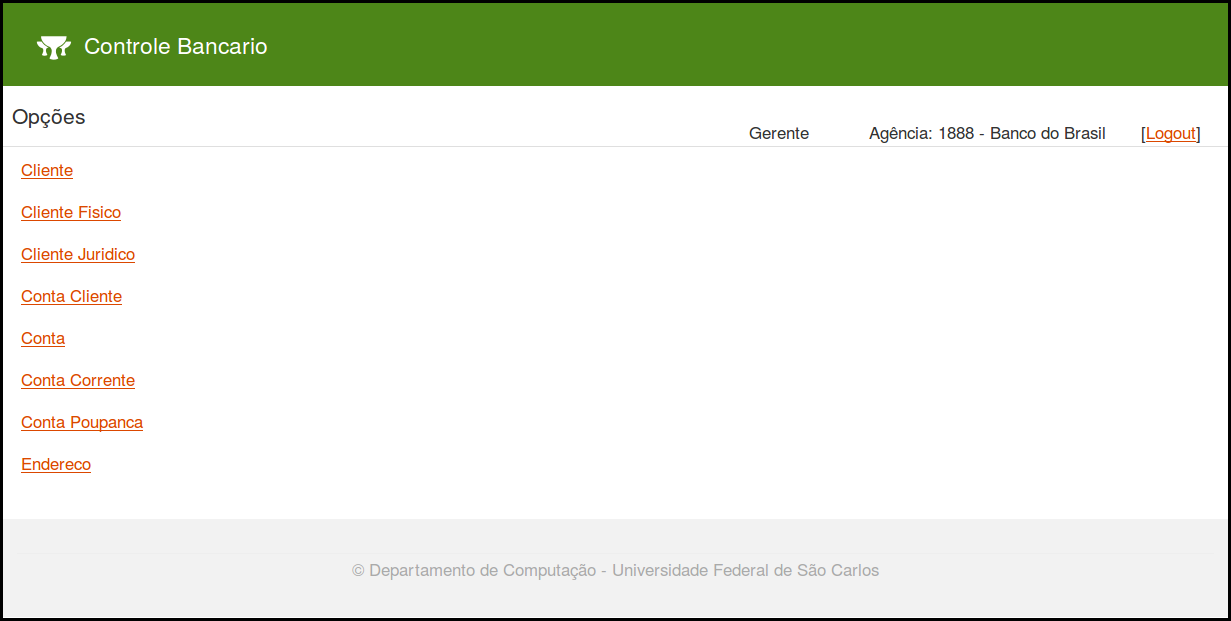
\includegraphics[width=12cm]{pageGerente}
\caption{Visão {\bf main/index.gsp}: {\bf ROLE\_GERENTE}}
\label{figPageGerente}
\end{figure}

Conforme pode-se  observar o  usuário {\it logado}  tem oito  opções disponíveis
(controladores da aplicação {\bf ControleBancario}): 

\vspace{0.3cm}

\begin{itemize}

\item  {\bf Cliente}, {\bf  ClienteFisico} e  {\bf ClienteJuridico}  caso deseje
  acessar/atualizar a lista de clientes; 

\vspace{0.3cm}

\item  {\bf  Conta},  {\bf  ContaCorrente}  e {\bf  ContaPoupança}  caso  deseje
  acessar/atualizar  a lista  de  contas  da agência  do  usuário {\it  logado}.
  Figura~\ref{indexContaFig} apresenta  a lista  de transações associadas  a uma
  conta do usuário {\it logado}; 

\vspace{0.3cm}

\item   {\bf   ContaCliente}   caso   deseje  acessar/atualizar   a   lista   de
  relacionamentos entre clientes e contas da agência do usuário {\it logado};

\vspace{0.3cm}

\item  {\bf  Endereco}  caso  deseje  acessar/atualizar  a  lista  de  endereços
  cadastrados.
 
\end{itemize}

\vspace{0.3cm}

\begin{figure}[htbp]
\centering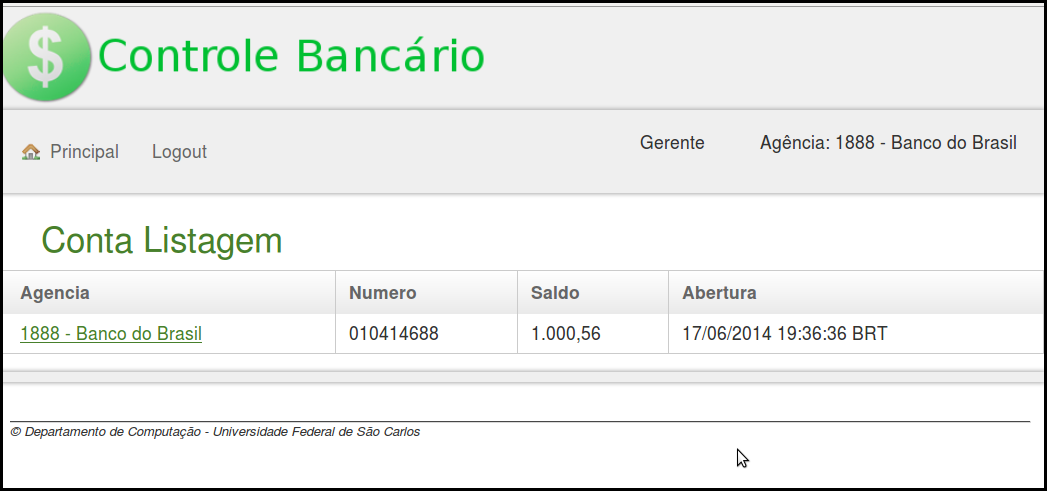
\includegraphics[width=12cm]{indexConta}
\caption{Lista de contas da agência do usuário {\it logado}}
\label{indexContaFig}
\end{figure}

\newpage

\section{Preenchimento automático de endereços}\label{secAutoFill}

\vspace{0.5cm}

Essa seção  tem como objetivo  incorporar, na aplicação  {\bf ControleBancario},
algumas funcionalidades AJAX  relacionadas ao acesso a um  serviço {\it web}. Em
especial,   essa  seção   apresenta   a  implementação   da  funcionalidade   de
preenchimento automático dos atributos da classe de domínio {\bf Endereco}. 

Ou seja, dado o atributo CEP,  os demais atributos desse classe de domínio serão
preenchidos automaticamente.  Para prover  essa funcionalidade, será acessado um
serviço {\it web} que, dado um CEP como parâmetro, retorna as demais informações
de um endereço (logradouro, bairro, cidade, etc).  

\subsection{Templates endereco/\_form.gsp \& endereco/\_address.gsp}

\vspace{0.5cm}

O primeiro passo na  implementação da funcionalidade de preenchimento automático
de  endereços consiste  em alterar  o {\it  template}  {\bf endereco/\_form.gsp}
conforme apresentado no Código~\ref{codEnderecoForm}.

Basicamente   foram  realizadas   duas   alterações  no   {\it  template}   {\bf
  endereco/\_form.gsp}.  A primeira  consiste em  alterar o  campo de  texto CEP
(linhas  8-10)  de  tal  forma  que  o  tratamento  ao  evento  Javascript  {\it
  onblur}\footnote{O evento {\it onblur} ocorre  quando um objeto perde o foco.}
consiste em invocar, passando como parâmetro o conteúdo do campo de texto CEP, a
ação {\bf addressByCEP()} do controlador {\bf EnderecoController}. 

\begin{lstlisting}[caption={\it Template} {\bf endereco/\_form.gsp}, frame=trBL,
    float=htbp, label=codEnderecoForm, numbers=left] 
<%@ page import="br.ufscar.dc.dsw.Endereco" %>
              
<div class="fieldcontain ${hasErrors(bean: enderecoInstance, field: 'CEP', 'error')} required">
 <label for="CEP">
  <g:message code="endereco.CEP.label" default="CEP" />
  <span class="required-indicator">*</span>
 </label>
 <g:textField name="CEP" maxlength="9" required="" value="${enderecoInstance?.CEP}" 
    onblur="${remoteFunction(action: 'addressByCEP', update: [success: 'addressContainer'],
                             params: '\'CEP=\' + this.value')}"/>
</div>

<div id="addressContainer">
    <g:render template="address"/>
</div>
\end{lstlisting}

A   segunda   alteração   consiste    em   inserir   o   {\it   template}   {\bf
  endereco/\_address.gsp} (Código~\ref{codEnderecoAddress}) que contem os demais
atributos  da  classe  de  domínio   {\bf  Endereco}.   O  {\it  template}  {\bf
  endereco/\_address.gsp} será atualizado em resposta ao retorno da invocação da
ação {\bf addressByCEP()} do  controlador {\bf EnderecoController}.  Ou seja, as
informações retornadas  pela ação {\bf  addressByCEP()} serão utilizados  para o
prenchimento  automático  dos  demais   atributos  da  classe  de  domínio  {\bf
  Endereco}.  

É importante salientar que  o {\it template} {\bf endereco/\_address.gsp} apenas
será atualizado pois encontra-se no escopo  de uma {\it tag} {\bf div} cujo {\bf
  id} ({\it addressContainer}) é igual ao valor do atributo {\bf update/success}
de {\bf remoteFunction()}. 

Uma segunda  observação é que  os campos {\bf  logradouro}, {\bf bairro}  e {\bf
  cidade}  no {\it  template} {\bf  endereco/\_address.gsp}  estão desabilitados
(não  podem ser  alterados).   Esses valores  serão preenchidos  automaticamente
pelas informações retornadas pela ação {\bf addressByCEP()}.  

\begin{lstlisting}[caption={\it    Template}    {\bf    endereco/\_address.gsp},
    frame=trBL, float=htbp, label=codEnderecoAddress] 
<%@ page import="br.ufscar.dc.dsw.Endereco" %>

<div class="fieldcontain ${hasErrors(bean: enderecoInstance, field: 'logradouro', 'error')} required">
	<label for="logradouro">
		<g:message code="endereco.logradouro.label" default="Logradouro" />
		<span class="required-indicator">*</span>
	</label>
	<g:textField name="logradouro" maxlength="30" required="" disabled value="${enderecoInstance?.logradouro}"/>
</div>

<div class="fieldcontain ${hasErrors(bean: enderecoInstance, field: 'numero', 'error')} required">
	<label for="numero">
		<g:message code="endereco.numero.label" default="Numero" />
		<span class="required-indicator">*</span>
	</label>
	<g:field name="numero" type="number" min="0" value="${enderecoInstance.numero}" required=""/>
</div>

<div class="fieldcontain ${hasErrors(bean: enderecoInstance, field: 'complemento', 'error')} ">
	<label for="complemento">
		<g:message code="endereco.complemento.label" default="Complemento" />
		
	</label>
	<g:textField name="complemento" maxlength="20" value="${enderecoInstance?.complemento}"/>
</div>

<div class="fieldcontain ${hasErrors(bean: enderecoInstance, field: 'bairro', 'error')} required">
	<label for="bairro">
		<g:message code="endereco.bairro.label" default="Bairro" />
		<span class="required-indicator">*</span>
	</label>
	<g:textField name="bairro" maxlength="20" required="" disabled value="${enderecoInstance?.bairro}"/>
</div>

<div class="fieldcontain ${hasErrors(bean: enderecoInstance, field: 'cidade', 'error')} required">
	<label for="cidade">
		<g:message code="endereco.cidade.label" default="Cidade" />
		<span class="required-indicator">*</span>
	</label>
	<g:select id="cidade" name="cidade.id" from="${br.ufscar.dc.dsw.Cidade.list()}" optionKey="id" required="" disabled value="${enderecoInstance?.cidade?.id}" class="many-to-one"/>
</div>
\end{lstlisting}

\newpage

\subsection{Controlador: EnderecoController}
\index{Serviços {\it web} REST!Cliente}

\vspace{0.5cm}

Código~\ref{codEnderecoController}  apresenta  a   implementação  da  ação  {\bf
  addressByCEP()} que,  conforme discutido  anteriormente, é invocado  pelo {\it
  template} {\bf endereco/\_form.gsp}. 

Essa  ação utiliza  o {\it  plugin} que  provê funcionalidades  para o  acesso a
serviços {\it web}.  Ou seja,  com a utilização das funcionalidades providas por
esse {\it plugin} é possível acessar serviços {\it web}.  

Conforme pode-se observar essa ação invoca um serviço {\it web} que, dado um CEP
como  parâmetro,  retorna as  demais  informações  de  um endereço  (logradouro,
bairro, cidade, etc). 

O serviço {\it  web} retorna o endereço em  formato JSON\footnote{JSON, acrônimo
  para {\it JavaScript  Object Notation}, é um formato  leve para intercâmbio de
  dados computacionais.} com as seguintes informações: 

\vspace{0.3cm}

\begin{itemize}

\item {\bf uf} que armazena a sigla da unidade federativa/estado;

\vspace{0.3cm}

\item {\bf cidade} que armazena o nome da cidade;

\vspace{0.3cm}

\item {\bf bairro} que armazena o nome do bairro;

\vspace{0.3cm}

\item {\bf  tipo\_logradouro} que armazena  o tipo do logradouro  (rua, avenida,
  etc); e

\vspace{0.3cm}

\item {\bf logradouro} que armazena o nome do logradouro.

\end{itemize}

\begin{lstlisting}[caption=Controlador  {\bf EnderecoController}, frame  = trBL,
    float=htbp, label=codEnderecoController] 
class EnderecoController {

    // Demais a^çõ^es/atributos/m^é^todos do controlador EnderecoController

    def addressByCEP() {
        def html
        
        try {
            withHttp(uri: "http://cep.republicavirtual.com.br/") {
                html = get(path : 'web_cep.php', 
                    query : [cep:params.CEP, formato:'json'])
            
                params.estado = Estado.findBySigla(html.uf)
                params.cidade = Cidade.findByNomeAndEstado(html.cidade, params.estado)
                params.bairro = html.bairro
                params.logradouro = html.tipo_logradouro + " " + html.logradouro
            }
        
               
            render template: 'address', model: [enderecoInstance: new Endereco(params)]
        } catch (Exception e) {
            println e
        }
    }
}
\end{lstlisting}

\vspace{0.3cm}

Tomando como base as informações retornadas  pelo serviço {\it web}, a ação {\bf
  addressByCEP()}  cria uma  instância da  classe  de domínio  {\bf Endereco}  e
retorna  essa   instância  para  ser   renderizada  pelo  {\it   template}  {\bf
  endereco/\_address.gsp}.

\newpage

Figura~\ref{figEnderecoCEP} apresenta a página de cadastro de um endereço (visão
{\bf endereco/create.gsp}) em que os  atributos {\bf logradouro}, {\bf bairro} e
{\bf cidade} foram preenchidos automaticamente pelas informações retornadas pela
ação {\bf addressByCEP()}.  

\vspace{0.3cm}

\begin{figure}[htbp]
\centering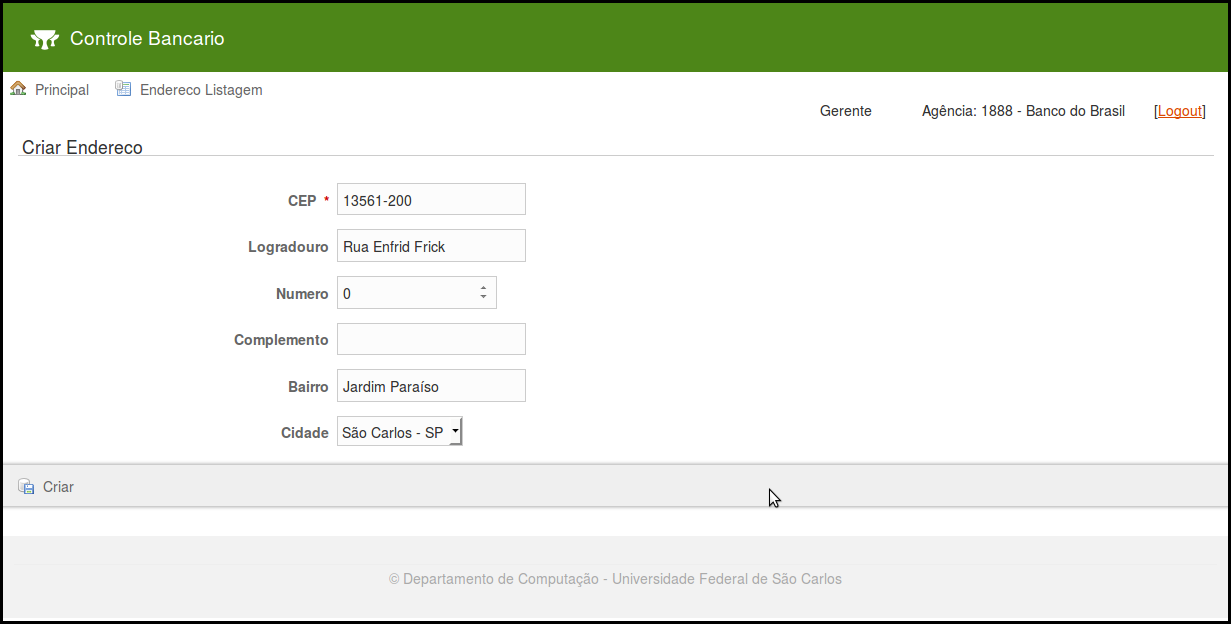
\includegraphics[width=13cm]{enderecoCEP}
\caption{Visão {\bf endereco/create.gsp}: Preenchimento automático de atributos}
\label{figEnderecoCEP}
\end{figure}

\section{Considerações finais}

\vspace{0.3cm}

Esse capítulo  apresentou a terceira  versão da implementação da  aplicação {\bf
  ControleBancario}.         O        código-fonte        dessa        aplicação
({\footnotesize\texttt{ControleBancarioV3.zip}}) encontra-se  disponível no {\it
  Moodle}         do        curso,        localizado         no        endereço:
{\footnotesize\url{http://moodle.latosensu.dc.ufscar.br}}. Seguindo os passos do
tutorial   apresentado   obtem-se   esse   mesmo  código   da   aplicação   {\bf
  ControleBancario}.  

Dando continuidade ao desenvolvimento em  Grails, o próximo capítulo apresenta a
implementação   de  novas   funcionalidades  no   contexto  da   aplicação  {\bf
  ControleBancario}.
